\section{硬件与性能基础}
\label{sec:background}

在深入理解Transformer架构之前,我们需要掌握现代硬件的性能模型。本节介绍Roofline模型及相关概念,这些知识对于理解后续章节中的效率优化技术(如FlashAttention、MoE)至关重要。

\subsection{Roofline Model}

Roofline模型是分析程序性能的经典框架,它通过三个基本约束来界定算法的性能上限:
\begin{itemize}
    \item 计算速度(FLOPs/秒)
    \item 数据传输带宽(字节/秒)
    \item 总内存容量
\end{itemize}

\begin{definition}[Arithmetic Intensity]
算术强度(Arithmetic Intensity)定义为单位数据传输所执行的计算量:
\begin{equation}
    \text{Arithmetic Intensity} = \frac{\text{Total FLOPs}}{\text{Total Bytes Transferred}}
    \label{eq:arithmetic_intensity}
\end{equation}
单位通常为 FLOPs/Byte。
\end{definition}

算术强度是判断程序瓶颈的关键指标。当算术强度高时,计算时间主导整体性能;当算术强度低时,内存带宽成为瓶颈。

\subsection{Memory Hierarchy}

现代加速器(GPU/TPU)存在明显的内存层次结构,不同层级的带宽和容量差异巨大:

\begin{table}[htbp]
\centering
\caption{GPU内存层次结构对比(以NVIDIA H100为例)}
\label{tab:memory_hierarchy}
\begin{tabular}{lccc}
\toprule
Memory Type & Capacity & Bandwidth & Latency \\
\midrule
Registers & $\sim$256KB/SM & $\sim$20 TB/s & 1 cycle \\
Shared Memory (SRAM) & 228KB/SM & $\sim$19 TB/s & $\sim$20 cycles \\
L2 Cache & 50MB & $\sim$12 TB/s & $\sim$200 cycles \\
HBM (Global Memory) & 80GB & 3.35 TB/s & $\sim$400 cycles \\
\bottomrule
\end{tabular}
\end{table}

这种层次结构意味着:
\begin{itemize}
    \item SRAM访问比HBM快约10倍
    \item 算法设计应尽量减少HBM访问,最大化数据复用
    \item FlashAttention等技术正是利用了这一特性
\end{itemize}

\subsection{Compute-bound vs Memory-bound}

程序的性能瓶颈可以分为两类:

\paragraph{计算时间与访存时间}
\begin{align}
    T_{\text{compute}} &= \frac{\text{FLOPs}}{\text{Peak FLOPs/s}} \\
    T_{\text{memory}} &= \frac{\text{Bytes}}{\text{Bandwidth (Bytes/s)}}
\end{align}

总执行时间的界限为:
\begin{equation}
    \max(T_{\text{compute}}, T_{\text{memory}}) \leq T_{\text{total}} \leq T_{\text{compute}} + T_{\text{memory}}
\end{equation}

\begin{definition}[Critical Arithmetic Intensity]
硬件的临界算术强度定义为:
\begin{equation}
    I_{\text{critical}} = \frac{\text{Peak FLOPs/s}}{\text{Memory Bandwidth (Bytes/s)}}
    \label{eq:critical_intensity}
\end{equation}
\end{definition}

\begin{itemize}
    \item 当 $I < I_{\text{critical}}$ 时,程序是 \textbf{Memory-bound},内存带宽是瓶颈
    \item 当 $I > I_{\text{critical}}$ 时,程序是 \textbf{Compute-bound},计算能力是瓶颈
\end{itemize}

\begin{figure}[htbp]
    \centering
    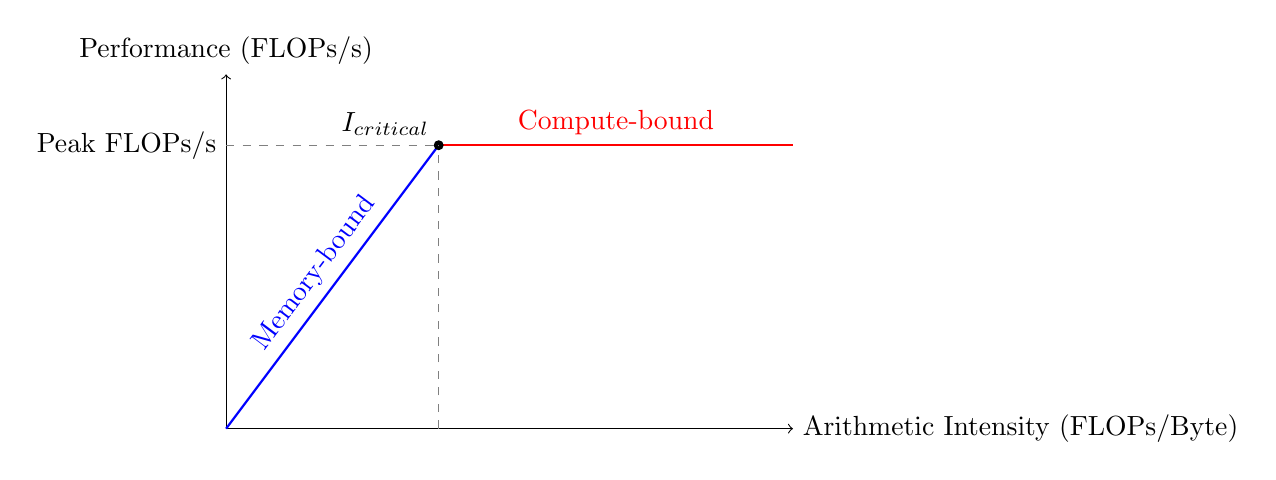
\begin{tikzpicture}[scale=0.9]
        % Axes
        \draw[->] (0,0) -- (8,0) node[right] {Arithmetic Intensity (FLOPs/Byte)};
        \draw[->] (0,0) -- (0,5) node[above] {Performance (FLOPs/s)};

        % Roofline
        \draw[thick, blue] (0,0) -- (3,4) node[midway, above, sloped] {Memory-bound};
        \draw[thick, red] (3,4) -- (8,4) node[midway, above] {Compute-bound};

        % Critical point
        \fill (3,4) circle (2pt) node[above left] {$I_{\text{critical}}$};

        % Peak lines (dashed)
        \draw[dashed, gray] (0,4) -- (3,4);
        \draw[dashed, gray] (3,0) -- (3,4);

        % Labels
        \node[left] at (0,4) {Peak FLOPs/s};
    \end{tikzpicture}
    \caption{Roofline模型示意图:性能受内存带宽和计算能力的双重约束}
    \label{fig:roofline}
\end{figure}

\subsection{Hardware Specifications}

表~\ref{tab:hardware_specs}列出了主流AI加速器的关键规格和临界算术强度。

\begin{table}[htbp]
\centering
\caption{主流AI加速器规格对比}
\label{tab:hardware_specs}
\begin{tabular}{lcccc}
\toprule
Hardware & Peak FLOPs/s (BF16) & HBM Bandwidth & $I_{\text{critical}}$ \\
\midrule
NVIDIA A100 & 312 TFLOPs & 2.0 TB/s & $\sim$156 \\
NVIDIA H100 & 990 TFLOPs & 3.35 TB/s & $\sim$296 \\
Google TPU v5e & 197 TFLOPs & 820 GB/s & $\sim$240 \\
AMD MI300X & 1,307 TFLOPs & 5.3 TB/s & $\sim$247 \\
\bottomrule
\end{tabular}
\end{table}

\subsection{Matrix Multiplication Analysis}

矩阵乘法是Transformer的核心计算。对于 $C = AB$,其中 $A \in \R^{B \times D}$,$B \in \R^{D \times F}$:
\begin{equation}
    \text{FLOPs} = 2BDF
\end{equation}
\begin{equation}
    \text{Bytes} = 2(BD + DF + BF) \quad \text{(以fp16/bf16计)}
\end{equation}
因此算术强度为:
\begin{equation}
    I = \frac{2BDF}{2(BD + DF + BF)} = \frac{BDF}{BD + DF + BF}
\end{equation}
当 $B \ll D, F$ 时(小batch场景),近似为:
\begin{equation}
    I \approx B
\end{equation}

这意味着:
\begin{itemize}
    \item 小batch推理通常是 memory-bound
    \item 增大batch size可以提高计算效率
    \item 对于H100,batch size需要超过$\sim$300才能充分利用计算能力
\end{itemize}

\begin{example}[Transformer推理分析]
考虑一个LLaMA-7B模型在H100上的推理:
\begin{itemize}
    \item 模型维度 $d = 4096$,FFN维度 $d_{ff} = 11008$
    \item 单token推理:$B = 1$,算术强度 $I \approx 1 \ll 296$,严重memory-bound
    \item Batch size = 512:$I \approx 512 > 296$,可以达到compute-bound
\end{itemize}
这解释了为什么大batch推理吞吐量更高。
\end{example}

\subsection{Implications for Transformer Design}

Roofline分析对Transformer的设计和优化有重要指导意义:

\paragraph{注意力机制}
在常见实现中,标准注意力会显式构建大小为 $n \times n$ 的注意力矩阵,并多次读写到HBM,导致HBM访存量随序列长度按 $O(n^2)$ 增长。因此在Roofline模型下,注意力计算是典型的memory-bound kernel。FlashAttention等优化方法通过将计算分块到片上SRAM,避免显式构建 $n^2$ 注意力矩阵并减少HBM读写,从而显著提升性能(详见Section~\ref{sec:flash_attention})。

\paragraph{KV Cache}
自回归生成时,KV cache的加载是主要瓶颈。MQA和GQA通过减少KV头数来降低内存访问量。

\paragraph{模型并行}
当模型过大无法放入单卡时,需要考虑:
\begin{itemize}
    \item \textbf{Tensor Parallelism}: 切分矩阵维度,增加通信但保持计算
    \item \textbf{Pipeline Parallelism}: 切分层,引入bubble但减少通信
    \item \textbf{Expert Parallelism (MoE)}: 专家分布在不同设备,需要all-to-all通信
\end{itemize}

\paragraph{混合精度}
使用INT8权重 + BF16激活时:
\begin{itemize}
    \item 权重加载字节数减半
    \item 算术强度翻倍
    \item 临界batch size降至原来的一半
\end{itemize}

理解这些硬件特性是设计高效Transformer系统的基础。

\subsection{Distributed Training and Sharding}

当模型规模超过单个加速器的内存容量时,需要将参数和计算分布到多个设备上。\textbf{Sharding}(分片)是将张量切分到设备网格上的核心技术。

\begin{definition}[Sharding]
给定一个全局形状为 $[I, J]$ 的张量 $A$ 和一个设备网格 $\mathcal{M}$ 包含轴 $X, Y$,分片记号 $A[I_X, J_Y]$ 表示:
\begin{itemize}
    \item 第一维 $I$ 沿网格轴 $X$ 切分
    \item 第二维 $J$ 沿网格轴 $Y$ 切分
    \item 每个设备持有形状为 $[I/|X|, J/|Y|]$ 的本地分片
\end{itemize}
\end{definition}

\paragraph{分片约束}
一旦某个网格维度被用于切分张量的某个维度,该网格维度就被"消耗",不能再用于同一张量的其他维度。

\subsection{Communication Primitives}

分布式计算中有四个核心通信原语。为便于分析,我们约定:
\begin{itemize}
    \item $V$:每设备本地参与通信的数据量(Bytes)
    \item $N$:参与通信的设备数
    \item $W$:每设备的有效互连带宽(Bytes/s)
    \item $\{U_X\}$:表示沿网格轴 $X$ 的未归约(unreduced)状态
\end{itemize}

\paragraph{AllGather:收集分片}
将分布在各设备的分片收集起来,使每个设备都获得完整数据。
\begin{equation}
    A[I_X, J] \xrightarrow{\text{AllGather}} A[I, J]
\end{equation}
\begin{verbatim}
  之前: D0:[A]    D1:[B]    D2:[C]    D3:[D]      每设备 V
  之后: D0:[ABCD] D1:[ABCD] D2:[ABCD] D3:[ABCD]   每设备 4V
\end{verbatim}
\begin{itemize}
    \item 输入:每设备持有 $V$(全局数据的 $1/N$)
    \item 输出:每设备持有 $N \cdot V$(完整副本)
    \item 通信量:每设备接收 $(N-1) \cdot V$
    \item 成本:$T \approx V/W$(ring算法下,带宽被充分利用)
\end{itemize}

\paragraph{ReduceScatter:归约后分发}
先对各设备数据求和(Reduce),再将结果切分到各设备(Scatter)。
\begin{equation}
    A[I, J]\{U_X\} \xrightarrow{\text{ReduceScatter}} A[I, J_X]
\end{equation}
\begin{verbatim}
  之前: D0:[A0,B0,C0,D0] D1:[A1,B1,C1,D1] D2:[A2,B2,C2,D2] D3:[A3,B3,C3,D3]
        (每设备持有完整但未归约的梯度)
  之后: D0:[ΣA] D1:[ΣB] D2:[ΣC] D3:[ΣD]
        (每设备持有1/4的归约结果,其中 ΣA = A0+A1+A2+A3)
\end{verbatim}
\begin{itemize}
    \item 输入:每设备持有 $V$(未归约,需要与其他设备的对应数据相加)
    \item 输出:每设备持有 $V/N$(归约结果的一个分片)
    \item 成本:$T \approx V/W$
    \item 典型用途:梯度聚合后分片存储(FSDP/ZeRO)
\end{itemize}

\paragraph{AllReduce:归约后广播}
对所有设备的数据求和,并将完整结果发送给每个设备。等价于 ReduceScatter + AllGather。
\begin{equation}
    A[I, J]\{U_X\} \xrightarrow{\text{AllReduce}} A[I, J]
\end{equation}
\begin{verbatim}
  之前: D0:[A0,B0,C0,D0] D1:[A1,B1,C1,D1] D2:[...] D3:[...]  每设备 V
  之后: D0:[ΣA,ΣB,ΣC,ΣD] D1:[ΣA,ΣB,ΣC,ΣD] D2:[...] D3:[...]  每设备 V
        (每设备都持有完整的归约结果)
\end{verbatim}
\begin{itemize}
    \item 输入:每设备持有 $V$(未归约)
    \item 输出:每设备持有 $V$(完整的归约结果)
    \item 成本:$T \approx 2V/W$(两步操作)
    \item 典型用途:DDP梯度同步
\end{itemize}

\paragraph{AllToAll:重新分片}
将数据从一种分片方式转换为另一种,相当于"转置"切分轴。
\begin{equation}
    A[I, J_X] \xrightarrow{\text{AllToAll}} A[I_X, J]
\end{equation}
\begin{verbatim}
  之前: D0:[A0,A1,A2,A3] D1:[B0,B1,B2,B3] D2:[C0,C1,C2,C3] D3:[D0,D1,D2,D3]
        (按"行"切分:每设备持有一整行)
  之后: D0:[A0,B0,C0,D0] D1:[A1,B1,C1,D1] D2:[A2,B2,C2,D2] D3:[A3,B3,C3,D3]
        (按"列"切分:每设备持有一整列)
\end{verbatim}
\begin{itemize}
    \item 输入:每设备持有 $V$(按 $J$ 维切分)
    \item 输出:每设备持有 $V$(按 $I$ 维切分,内容不同但大小相同)
    \item 通信量:每设备发送 $(N-1)/N \cdot V \approx V$,接收同量
    \item 成本:$T \approx V/W$
\end{itemize}

\paragraph{四种通信原语对比}

\begin{table}[htbp]
\centering
\caption{通信原语完整对比($N=4$ 设备,每设备本地数据量 $V$)}
\label{tab:comm_comparison}
\begin{tabular}{lcccc}
\toprule
 & AllGather & ReduceScatter & AllReduce & AllToAll \\
\midrule
数据变化 & 分片$\to$完整 & 完整$\to$分片 & 完整$\to$完整 & 分片$\to$分片 \\
输入大小 & $V$ & $V$ & $V$ & $V$ \\
输出大小 & $N \cdot V$ & $V/N$ & $V$ & $V$ \\
是否归约 & 否 & 是 & 是 & 否 \\
通信成本 & $V/W$ & $V/W$ & $2V/W$ & $V/W$ \\
典型用途 & TP激活收集 & ZeRO梯度分片 & DDP梯度同步 & MoE路由 \\
\bottomrule
\end{tabular}
\end{table}

关键洞察:
\begin{itemize}
    \item \textbf{AllGather}:收集分片,每设备获得相同的完整副本
    \item \textbf{ReduceScatter}:归约后分片,每设备获得不同的归约结果分片
    \item \textbf{AllReduce}:归约后广播,每设备获得相同的完整归约结果(= ReduceScatter + AllGather)
    \item \textbf{AllToAll}:重新分片,每设备获得不同的数据(不归约,仅重分布)
\end{itemize}

\paragraph{AllToAll 在 MoE 中的应用}
MoE(Mixture of Experts)是 AllToAll 的典型应用场景。假设 $N$ 个设备各持有一个 Expert:

\begin{enumerate}
    \item \textbf{Router} 决定每个 token 应由哪个 Expert 处理
    \item \textbf{Dispatch}(AllToAll):将 token 发送到目标 Expert 所在设备
    \item \textbf{Expert 计算}:每设备用本地 Expert 处理收到的 token
    \item \textbf{Combine}(AllToAll):将结果发回原设备
\end{enumerate}

AllToAll 使得 token 能够高效地"找到"分布在不同设备上的 Expert,而无需在每个设备上复制所有 token。

\subsection{Distributed Matrix Multiplication}

分布式矩阵乘法 $C = AB$ 的通信策略取决于输入的分片模式:

\paragraph{Case 1: 非收缩维分片(无通信)}
\begin{equation}
    A[I_X, J] \cdot B[J, K_Y] \to C[I_X, K_Y]
\end{equation}
输出自动继承输入的分片模式,无需通信。

\paragraph{Case 2: 单输入收缩维分片(AllGather)}
\begin{equation}
    A[I, J_X] \cdot B[J, K] \xrightarrow{\text{AllGather}} A[I, J] \cdot B[J, K] \to C[I, K]
\end{equation}
需要先AllGather移除 $A$ 的分片。

\paragraph{Case 3: 双输入同轴收缩维分片(AllReduce)}
\begin{equation}
    A[I, J_X] \cdot B[J_X, K] \to C[I, K]\{U_X\} \xrightarrow{\text{AllReduce}} C[I, K]
\end{equation}
本地矩阵乘法产生部分和,AllReduce完成归约。

\paragraph{Case 4: 双输入同轴非收缩维分片(非法)}
\begin{equation}
    A[I_X, J] \cdot B[J, K_X] \to \text{Invalid (diagonal result)}
\end{equation}
必须先AllGather其中一个输入。

\begin{example}[策略选择]
对于 $C = AB$,其中 $A \in \R^{B \times D}$,$B \in \R^{D \times F}$,比较两种策略:

\textbf{策略1}(AllGather优先):
\begin{equation}
    T_1 = \underbrace{\frac{2DF}{W}}_{\text{AllGather } B} + \underbrace{\frac{2BDF}{C}}_{\text{Compute}}
\end{equation}

\textbf{策略2}(AllReduce优先):
\begin{equation}
    T_2 = \underbrace{\frac{4BF}{W}}_{\text{AllReduce } C} + \underbrace{\frac{2BDF/X}{C}}_{\text{Local Compute}}
\end{equation}

当 $D > 2X$(模型维度远大于并行度)时,策略2更优。
\end{example}

\subsection{Parallelism Strategies}

大规模Transformer训练通常结合多种并行策略:

\paragraph{Data Parallelism (DP)}
将batch维度切分到多个设备,每个设备持有完整模型副本:
\begin{itemize}
    \item 前向传播:各设备独立计算
    \item 反向传播:AllReduce同步梯度
    \item 优点:实现简单,通信量与模型大小成正比
    \item 缺点:内存冗余(每设备存完整模型)
\end{itemize}

\paragraph{Fully Sharded Data Parallelism (FSDP/ZeRO)}
将参数、梯度、优化器状态都沿数据维度切分:
\begin{equation}
    \text{Memory/device} = \frac{\text{Model Size}}{N_{\text{devices}}} + \text{Activations}
\end{equation}
计算前AllGather参数,计算后ReduceScatter梯度。

\paragraph{Tensor Parallelism (TP)}
将矩阵维度切分,每层内部并行计算:
\begin{itemize}
    \item Column Parallel:$W[D, F_X]$,前向AllGather,反向ReduceScatter
    \item Row Parallel:$W[D_X, F]$,前向ReduceScatter,反向AllGather
\end{itemize}
通常在Transformer的Attention和FFN中交替使用,每层需要2次AllReduce。

\paragraph{Pipeline Parallelism (PP)}
将模型层切分到不同设备,形成流水线:
\begin{itemize}
    \item 优点:通信量少(仅传递激活值)
    \item 缺点:存在流水线气泡(bubble),降低硬件利用率
    \item 优化:1F1B调度、交错调度等减少bubble
\end{itemize}

\paragraph{Expert Parallelism (EP)}
MoE模型中,不同专家分布在不同设备:
\begin{equation}
    \text{Input}[B, D] \xrightarrow{\text{AllToAll}} \text{Expert}_i[B_i, D] \xrightarrow{\text{Compute}} \xrightarrow{\text{AllToAll}} \text{Output}[B, D]
\end{equation}
需要AllToAll进行token路由和结果收集。

\paragraph{Sequence Parallelism (SP)}
将序列维度切分,与TP配合使用:
\begin{itemize}
    \item LayerNorm和Dropout沿序列维度切分
    \item 减少激活值内存
    \item 与TP共享通信,无额外开销
\end{itemize}

\subsection{Communication-Computation Overlap}

高效的分布式系统通过重叠通信和计算来隐藏通信延迟:

\begin{equation}
    T_{\text{total}} = \max(T_{\text{compute}}, T_{\text{comm}}) \quad \text{(理想情况)}
\end{equation}

实现技术:
\begin{itemize}
    \item \textbf{异步通信}:在计算进行时启动下一次通信
    \item \textbf{分块流水线}:将大张量切分为小块,交替计算和通信
    \item \textbf{梯度累积}:多个micro-batch累积后再同步
\end{itemize}

理解这些分布式并行技术是扩展Transformer到千亿参数规模的关键。
